\chapter{\chapvname}
\label{chapter5}
\section*{Overview}
This work presents portable, low-cost hardware for pressure mapping using EIT-based soft sensors. An important part of developing these EIT-based pressure sensors is the sensor characterisation as shown in the previous chapter. Therefore, this chapter also provides the design of a system required for characterising and validating the spatial, pressure, and temporal performance of different soft sensor material domains. The system is capable of driving soft EIT-based sensors using a range of sensing materials, shapes, and configurations. The hardware allows for the wireless transmission of EIT data to a remote device. 
A data capture frame rate of 12.7 Hz allows for the analysis of dynamic events. The maximum current drive voltage is $\pm$22 V and a voltage read resolution of $\pm$0.3 $\mu V$ allowing for a range of sensing domain sizes, thicknesses, and materials. A Cartesian force applicator device has been developed for the automatic characterisation which can apply and sense loads from 0 to 100 N with a resolution of $\pm$50 mN at rates of 0 - 800 mm/min. Loads can be applied in the $xy$ plane with an error of $\pm$0.01 mm. A standardised method has been provided for researchers to experiment with a range of different sensing domain materials and shapes. The system described in this work is suitable for both research and practical applications, making it a valuable tool for advancing the field of novel EIT-based soft pressure mapping sensor technology. All of the hardware and software for the ERT electronics module and Cartesian force applicator designs developed in this work are open-source and supplied in the supplementary material \cite{Ellingham2025}. 
To the best of the author's knowledge, no system for characterising soft EIT-based pressure mapping sensors in real-time has been presented in the literature at the time of writing this chapter.



\section{Introduction}
% TO DO: redo introduction in a regular format:
% 1. Impact sentence
% 2. Highlight research gaps
% 3. Introduce research 'solution'
To apply the pressure mapping sensor analysis and technology given in the previous chapter to a real world scenario, often portability, development time, and cost become an issue. More importantly there is no commercial product specifically made for soft conforming pressure mapping sensors. To combat this, a novel application specific EIT module has been created in this work for developing EIT-based pressure mapping sensors. In parallel there lacks a commercial system which can simulataneously gather compressive spatio-temporal stress-strain data for characterising the EIT-based pressure sensor technology developed. Hence a Cartesian force applicator has been designed for the purpose of researching and comparing the electromechanical properties of a range of potential sensing domain materials. 

% 4. Further background research
Electrical impedance tomography (EIT) is an imaging technique used to map impedance/resistance throughout a material using multiple boundary electrodes. The boundary electrodes inject current through the homogeneous domain instead of a patterned or layered one, allowing the sensor measurements to be non-invasive. 

EIT is most commonly used for thorax imaging for clinical respiratory analysis; however, this same method can be used for a multitude of applications with conductive bodies to map changes in impedance/resistance as shown in the previous chapter. Commercial devices that perform EIT, or the DC equivalent electrical resistivity tomography (ERT), exist in large-form factors such as Pulmovista 500 (Draeger, Luebeck, Germany), EIT16/32 (Sciospec Scientific Instruments GmbH, Leipzig, Germany), LuMon (Sentec, Lincoln, USA), Zeta (Zonge International, Tucson, USA), WGMD-4 (WTS Geophysical, Wanchai, Hong Kong). All of these options are application-specific for research, biomedical, and geophysical applications. Several research papers \cite{Chen2023,Hong2015,Lee2020,Li2023,Soleimani2006,Suh2022,Tiwari2022,Xu2022,Zhang2015,Zhang2016} have described similar but smaller versions of the commercial products mentioned.

In this work similar physical principles used in bio-medical and geophysical sensing are used to map localised compressive loads on a soft piezoresistive material. A core limiting factor of current pressure mapping technology is the lack of customisability in sensor size, shape, sensing domain material softness, and sensing material composition \cite{Gilanizadehdizaj2022,Rossiter2005,Liang2015,Fu2020}. Most often, pressure sensors are given in a rectangular format because of the arrays of wiring and sensing elements required within the sensing domain. EIT-based pressure mapping sensors are not constrained by wires or complex patterning within the sensing domain area. EIT-based pressure sensors can have a homogeneous sensing domain configured in various shapes. 

When refering to the circuitry capturing data for an EIT reconstruction the term ERT is used to show the circuit function. However, when refering to the reconstruction computer and resistance images generated the term EIT is used, as these can be generalised for complex impedances.
%Although the sensor described in this work as with many other previous works generates resistance images of the sensor domain, the term EIT instead of ERT for such sensors is often used as to not confuse these devices with typical ERT sensors, which are ubiquitous in large scale geological measurements.
%	\begin{figure}[H]
%		\centering
%		\includegraphics[width=0.30\linewidth]{Figures/picture showing future application.png} % same sketch style as the literature review sketch. sketch of person with prosthetic arm and with smart soles??
%		\caption{Potential future application of sensor technology}
%		\label{fig:future_app}
%	\end{figure}
To advance the research of this soft pressure mapping platform technology, we require a system that is lost cost, open source, easy to use, portable, and sufficiently flexible to test a range of different sensing domain materials. The system developed in this work is for the research and development of EIT-based pressure mapping sensors.
\begin{figure}[H]
	\centering
	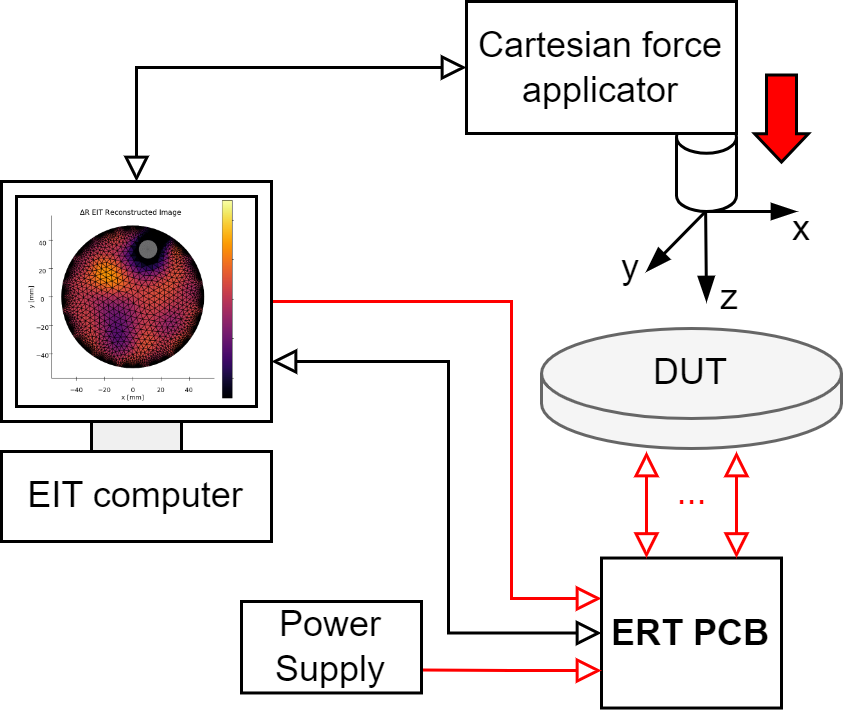
\includegraphics[width=0.5\linewidth]{Figures/ERT_PCB_and_CFA_system_simple.png}
	\caption{System architecture of ERT sensor and CFA setup. The large red arrow shows the direction of the force applicator compression onto the sensing domain (DUT) and analogue/power signals are shown with red arrows and digital signals with black arrows.}
	\label{fig:ERT_PCB_CFA_archit}
\end{figure}
The hardware of our system has two key components, a circuit for gathering raw ERT data and a Cartesian force applicator (CFA) machine for characterising an ERT-based pressure mapping sensor. The system characterises the sensor and can be used for validating the spatial, pressure, and temporal performance for different piezoresistive sensor material domains. The CFA allows for repeatable experiments and quantifiable data for different sensor configurations.



\section{Design Methodology and Analysis} 
An EIT-based pressure mapping sensor toolbox as been created that reliably and repetitively collects data for EIT-based pressure mapping and quantification of the sensor performance. The overall system is simple to construct and easy to operate and is split into the subsystems given in Figure \ref{fig:ERT_PCB_CFA_archit}. The build instructions for both subsystems are given in Appendix \ref{appendix-E}.

% ert sensor
The ERT sensor consists of an ERT sensor circuit and the sensing domain under test (DUT). The ERT circuit drives the EIT measurements through the sensing domain soft elastomer composite material. The ERT circuit designed is small (79 $\times$ 94 $\times$ 12 mm) for potential use in space-constrained mobile applications. 
The system has a programmable current source which can drive up to 50 mA of constant current. The voltage measurement circuit has an ADC resolution of 0.3 $\mu$V, ensuring that the small signals generated by small localised loads can be detected. The sensing domain in this work is a soft piezoresistive composite made from carbon black (CB) powder and silicone rubber with 16 boundary electrodes made from gold pins and copper tape, as seen in Figure \ref{fig:CBSR_samples_examples}. A sample containing the gold pin electrodes is also shown in Figure \ref{fig:ert_sensor} connected to the ERT data acquisition electronics.
\begin{figure}[H]
	\centering
	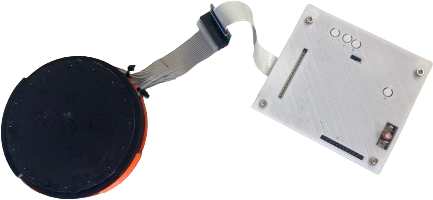
\includegraphics[width=0.6\linewidth]{Figures/ert_pcb_and_DUT.png}
	\caption{A soft sensor domain connected to the ERT sensor electronics.}
	\label{fig:ert_sensor}
\end{figure}
% cfa
To ensure that the sensor can accurately locate pressure points and their magnitude, the CFA device described in this work is used to apply compressive forces at various locations. The CFA test bed allows for loads within a 220 $\times$ 180 mm area.
\begin{figure}[H]
	\centering
	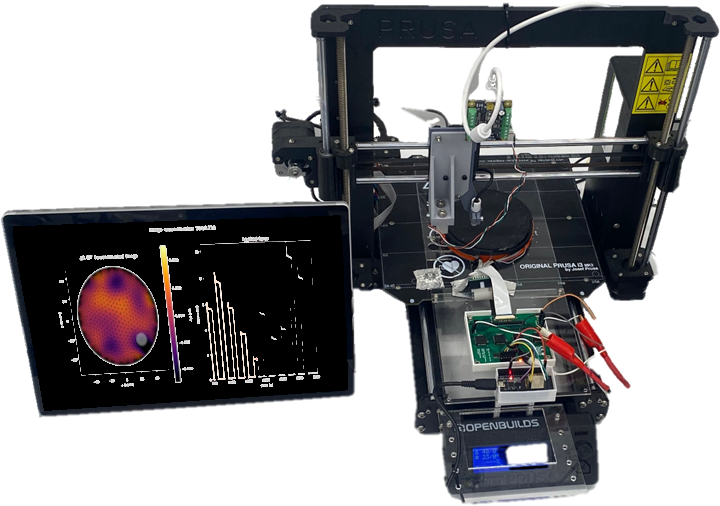
\includegraphics[width=0.6\linewidth]{Figures/cfa_screen_pic.png}
	\caption{Cartesian force applicator setup with an ERT circuit and EIT reconstruction computer}
	\label{fig:cfa_setup}
\end{figure} 
Previous research groups have developed EIT hardware for pressure mapping sensors \cite{Chen2023,Zhang2017b,Visentin2016,Yoon2017,Sun2020}; however, a complete open-source system including validation hardware has not yet been published. 


\begin{figure}[H]
\centering
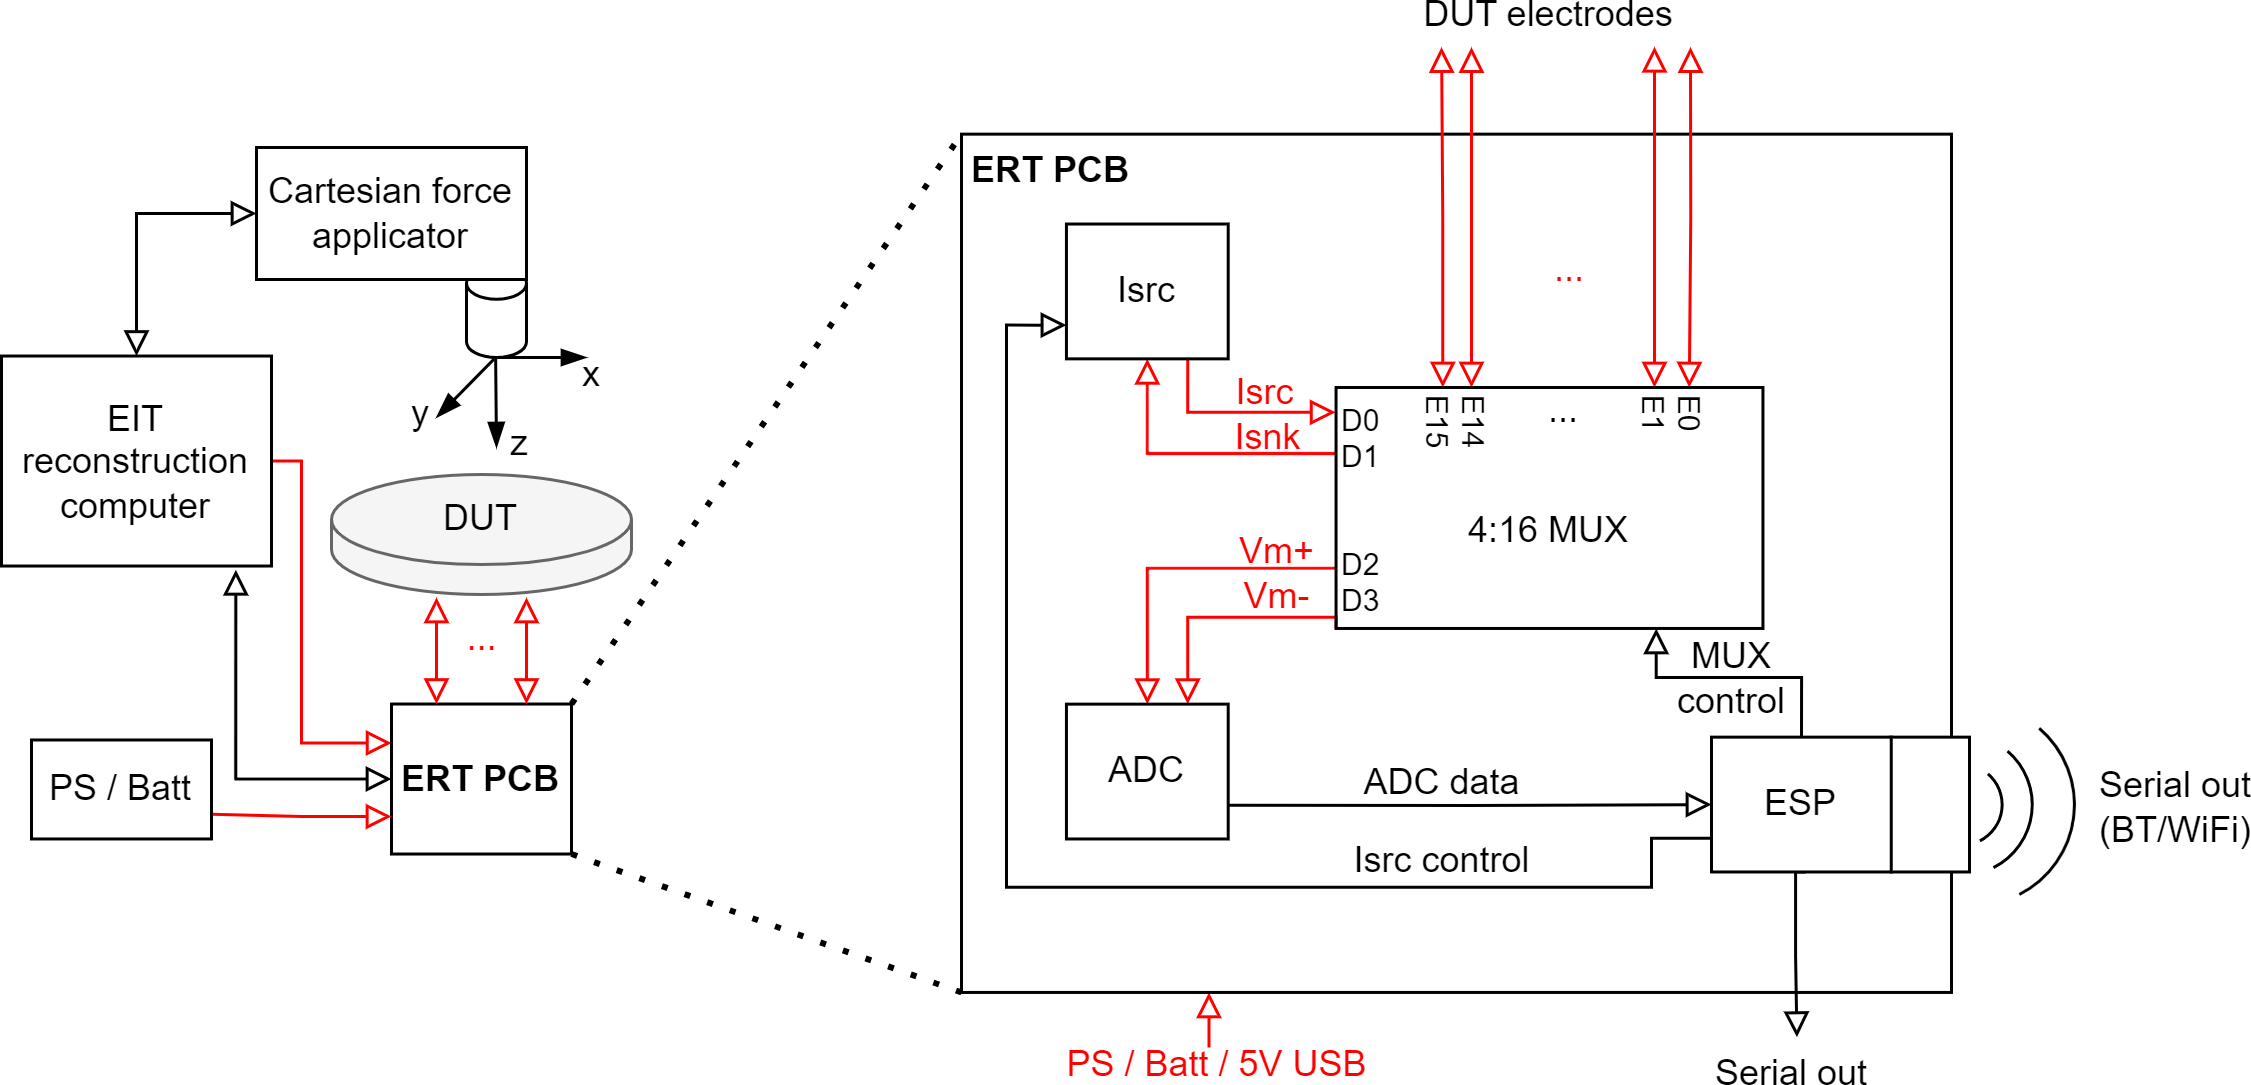
\includegraphics[width=\linewidth]{Figures/ERT_PCB_and_CFA_system.png}
\caption{System architecture of ERT sensor and CFA setup (left) and the key internal electrical signals of the ERT circuit (right). With analogue/power signals shown with red arrows and digital signals with black arrows.}
\label{fig:ERT_PCB_CFA_archit_full}
\end{figure}


\subsection{EIT cycle and load sequence}
While a sequence of compressive loads are applied by the CFA to the sensing domain, concurrently the ERT sensor circuit gathers data for EIT reconstruction. This cyclic EIT data capture process follows a specific sequence, 
\begin{figure}[H]
\centering
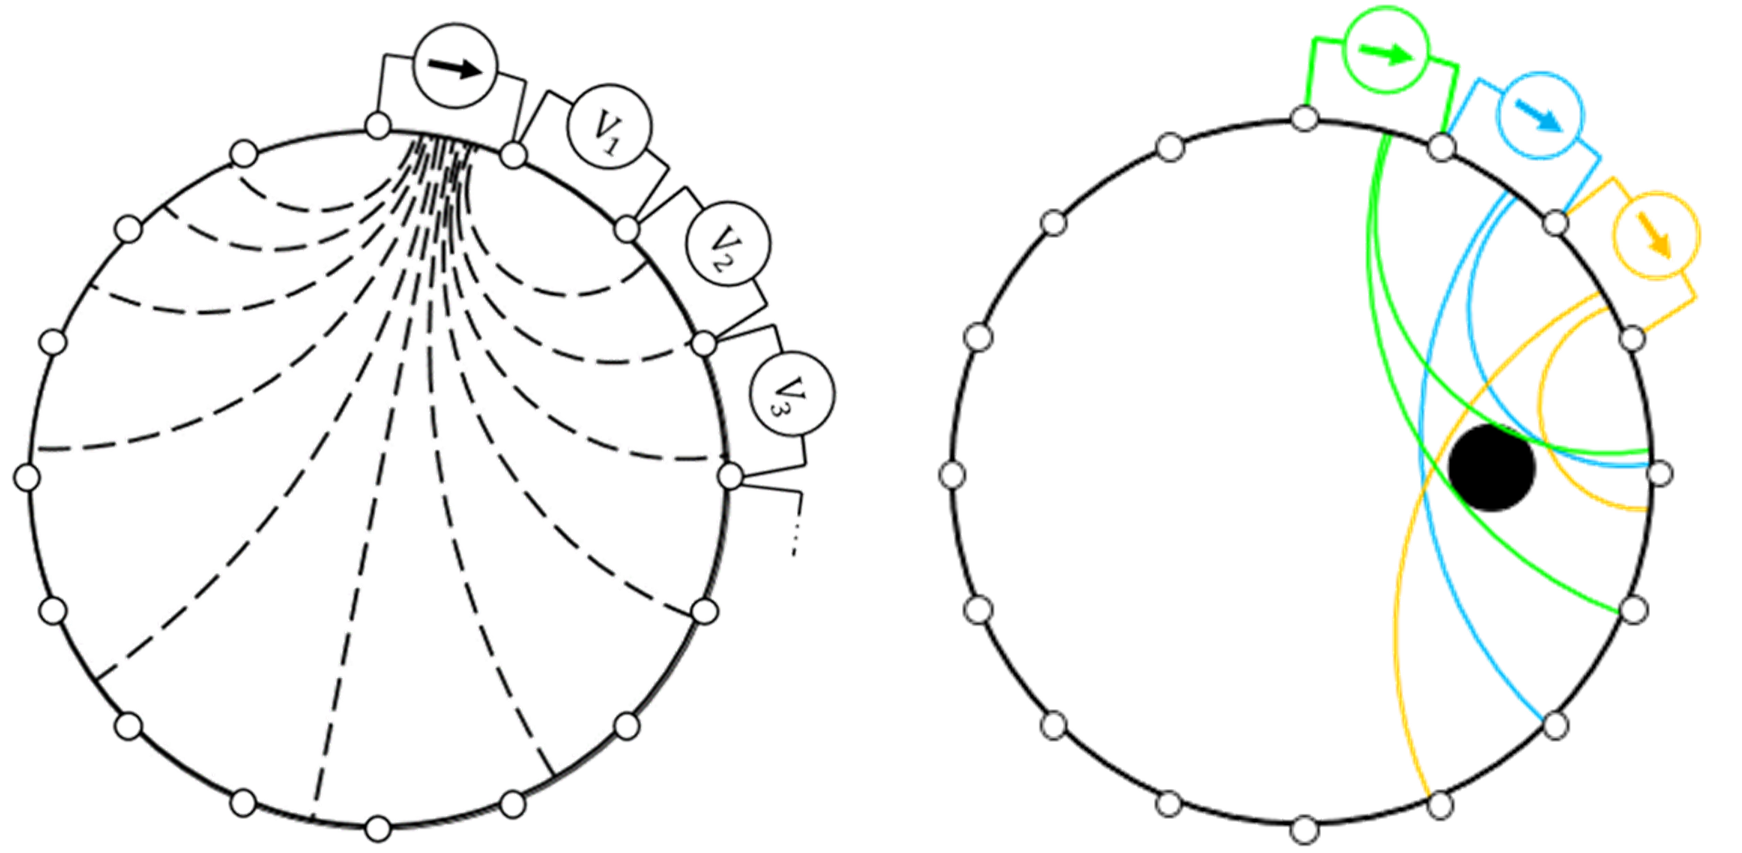
\includegraphics[width=0.8\linewidth]{Figures/eit_sequence.png}
\caption{EIT adjacent drive pattern sequence.}
\label{fig:EIT_adj_drive}
\end{figure}
\begin{enumerate}
\item A constant current is applied at adjacent electrode positions $E_i$ and $E_{i+1}$, these electrode positions are selected with the `MUX control' line.
\item Sequentially 16 adjacent electrode voltage measurements are completed next, again the electrode positions are selected with the `MUX control' line.
\item Each raw voltage measurement is transmitted through `serial out' to an `EIT reconstruction computer'.
\item The next current injection electrode position is selected, i.e. i = i + 1. Once all 16 current injection positions are completed, 256 voltages are measured giving enough data for one reconstruction frame. This is repeated for the duration of the experiment.
\end{enumerate}
Multiplexing of the voltage measurements was chosen instead of the alternative option of simultaneous voltage measurement, to maintain a low-cost circuit. The simultaneous voltage measurement solution involves 16 separate ADCs, one for each electrode. A DC current source was chosen instead of the AC alternative because the sensing domains do not show significant changes in reactance during loading events. The hardware allows for the loading sequence to be altered and optimised for the sensing domain and application, because of the four independently switchable multiplexers controlling the current source and voltage reading electrodes.


\subsection{Small signal measurement}
% important because precision measurements required for EIT.
The range of voltages required for reconstructing minute changes in resistances of a sensing domain spans several orders of magnitudes in EIT systems. Therefore a high dynamic range, high resolution, low-noise voltage measurement system is required to accurately capture this data.

% Include resistor mesh network validation for range of expected votlages?
To evaluate the performance of the system with a standardised testing domain a resistor mesh network was created. The mesh network was created to validate the expected resolution required for generating EIT reconstructions \cite{Ellingham2022} for a variety of different resistances and resistance changes. The resistor mesh network provided a standardised platform with known resistor values and tolerances for the comparison a real and simulated resistor mesh network. The resistor mesh network was chosen to provide a range EIT voltage data comparable to that of the real CBSR composite material.

A script was created to form a square resistor mesh network of various dimensions and various background resistance values. PySpice circuit simulator \cite{PySpice2021} was used to run a zero noise simulation on the system to show the expected difference in raw ERT voltage data between a homogeneous resistor mesh and a resistor mesh with an anomalous blob as shown in Figure \ref{fig:vdiff_res_mesh}. The maximum and minimum $\Delta V_{read}$ values shown in Figure \ref{fig:vdiff_res_mesh} and 94.994 mV and 53 $\mu$V respectively.
\begin{figure}[H]
\centering
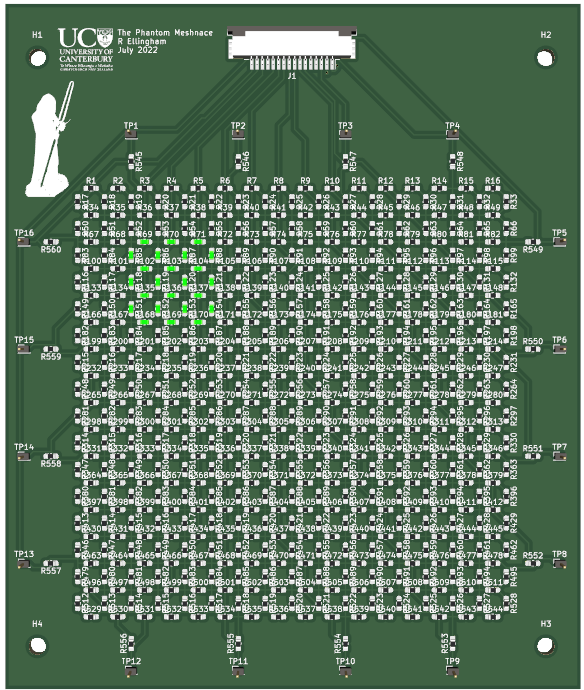
\includegraphics[width=0.32\linewidth]{Figures/res_mesh_pcb.png}
\hspace{1cm}
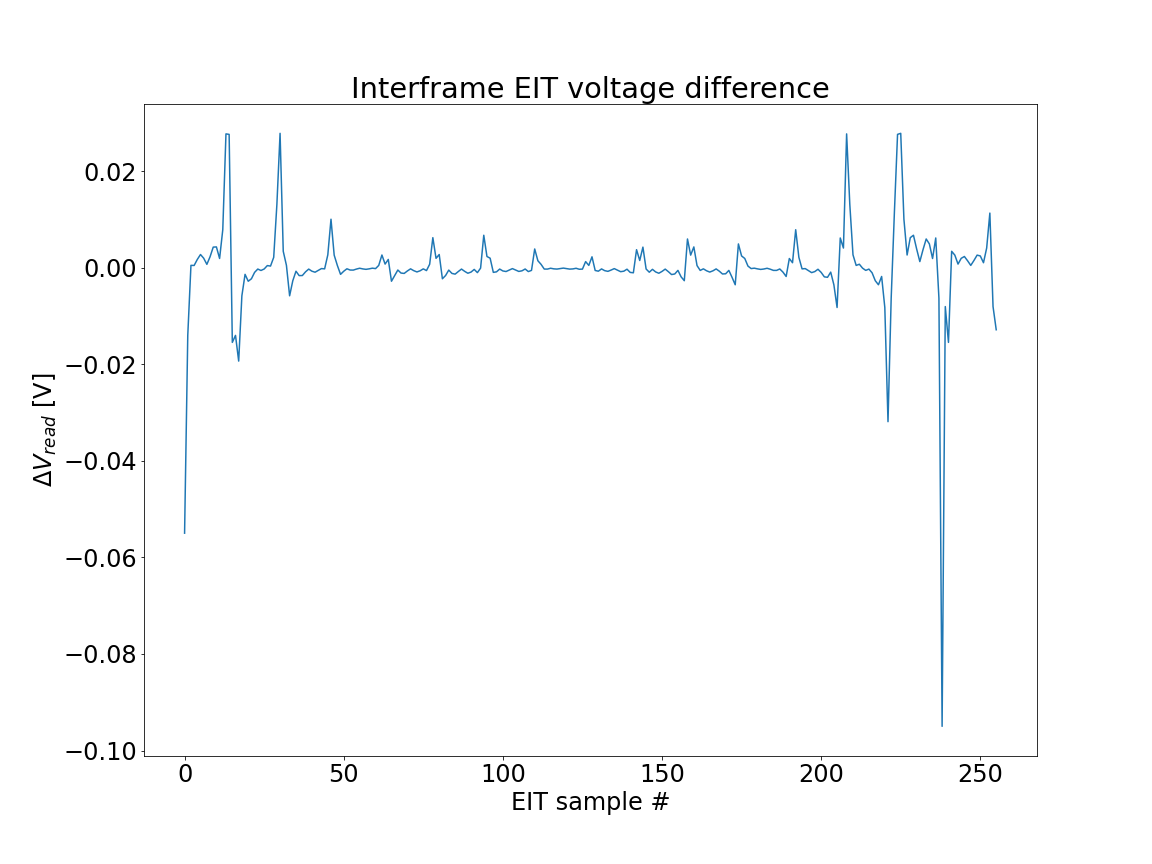
\includegraphics[width=0.56\linewidth]{Figures/EIT_Vdiff_res_mesh_2k2bg_3k3anom.png} % TODO: change this to a dotted plot as these values shouldn't be linked.
\caption{Left: A resistor mesh network for validating the ERT circuit, with the anomalous resistors highlighted in green. Right: The difference between EIT raw voltage data from a homogeneous square 2.2 k$\Omega$ resistor mesh domain and the same domain with a 3.3 k$\Omega$ resistor mesh anomaly.}
\label{fig:vdiff_res_mesh}
\end{figure}

It is non-trivial to determine the exact resolution required for an EIT based pressure mapping sensor voltage measurements as it depends on the inherent noise of the domain, the force resolution required, the expected external noise, the drive current, the EIT reconstruction algorithm used, amongst other factors. This work uses a 24 bit ADC so that given an ideal noiseless representative domain the minimum voltage data shown in Figure \ref{fig:vdiff_res_mesh} will be an order of magnitude larger than the resolution of the ADC.


\subsection{Signal generation}
% quantify and discuss importance of the isrc circuit..
To ensure a range of soft piezoresistive sensing domains can be tested a range of current source values are required to detect voltage ranges within detectable range of the circuit's ADCs. The current source can drive a current, $I_{src}$ between 15 $\mu$A and 50 mA and can be set as a programmable or fixed current source value. The $I_{src}$ value can be altered by changing the $R_{Isrc}$ [R7 or R8] value as shown in Equation \ref{eqn:isrc}.
\begin{equation}
I_{src} = \frac{0.617}{R_{Isrc}} + 15 \space \mu A
\label{eqn:isrc}
\end{equation}
If a fixed current source is desired for the ERT circuit $R_{Isrc}$ sets the current source value based on Equation \ref{eqn:isrc}. If the circuit is configured as a programmable current source, the digital potentiometer [U9] controlling the $R_{Isrc}$ value can be increased in 39 $\Omega$ increments up to a maximum of 10 k$\Omega$ or a high impedance state. The possible programmable current source values are given in the \verb|isrc_lookup.xlsx| file in the repository. If the resistivity of the domain is too high the current source supply will saturate to Vs. Ensure the domain resistivity is sufficiently low for this current source driving voltage supply saturation not to occur within its expected range of use. 
A sufficiently high current value must pass through the domain to ensure low noise readings throughout the boundary electrodes on the domain. This noise predominantly occurs due to electrostatic effects in sensing domains. To ensure this current can be driven for the sensor domain configuration given in this work, a supply voltage, $\pm V_s$, of $\pm$20 V should be used.


\subsection{Signal conditioning}
% quantify and discuss importance of the opamp circuit and opamp selection. input bias current, Voffset etc...
To help ensure that voltage generated by the current injection across a range of piezoresistive sensing domains can be read by the circuit's ADCs, an signal conditioning circuit is required.
When using the recommended supply voltage of $\pm$20 V, an attenuation stage is required for the input into the ADC. This is done with an operational amplifier (opamp) voltage buffer-divider-buffer circuit as shown in Figure \ref{fig:opamp_ckt}. When using a single ended 5 V supply to drive the current source this opamp circuit can be bypassed using the jumpers shown in Figure \ref{fig:ert_pcb_pinout_mode} as the attenuation is not required and the offset and noise due to the opamp circuit can be avoided. However due to a lack of a negative $Vss$, the multiplexer channel resistance will be degraded as exemplified in Figure \ref{fig:mux_r_on}.
\begin{figure}[H]
\centering
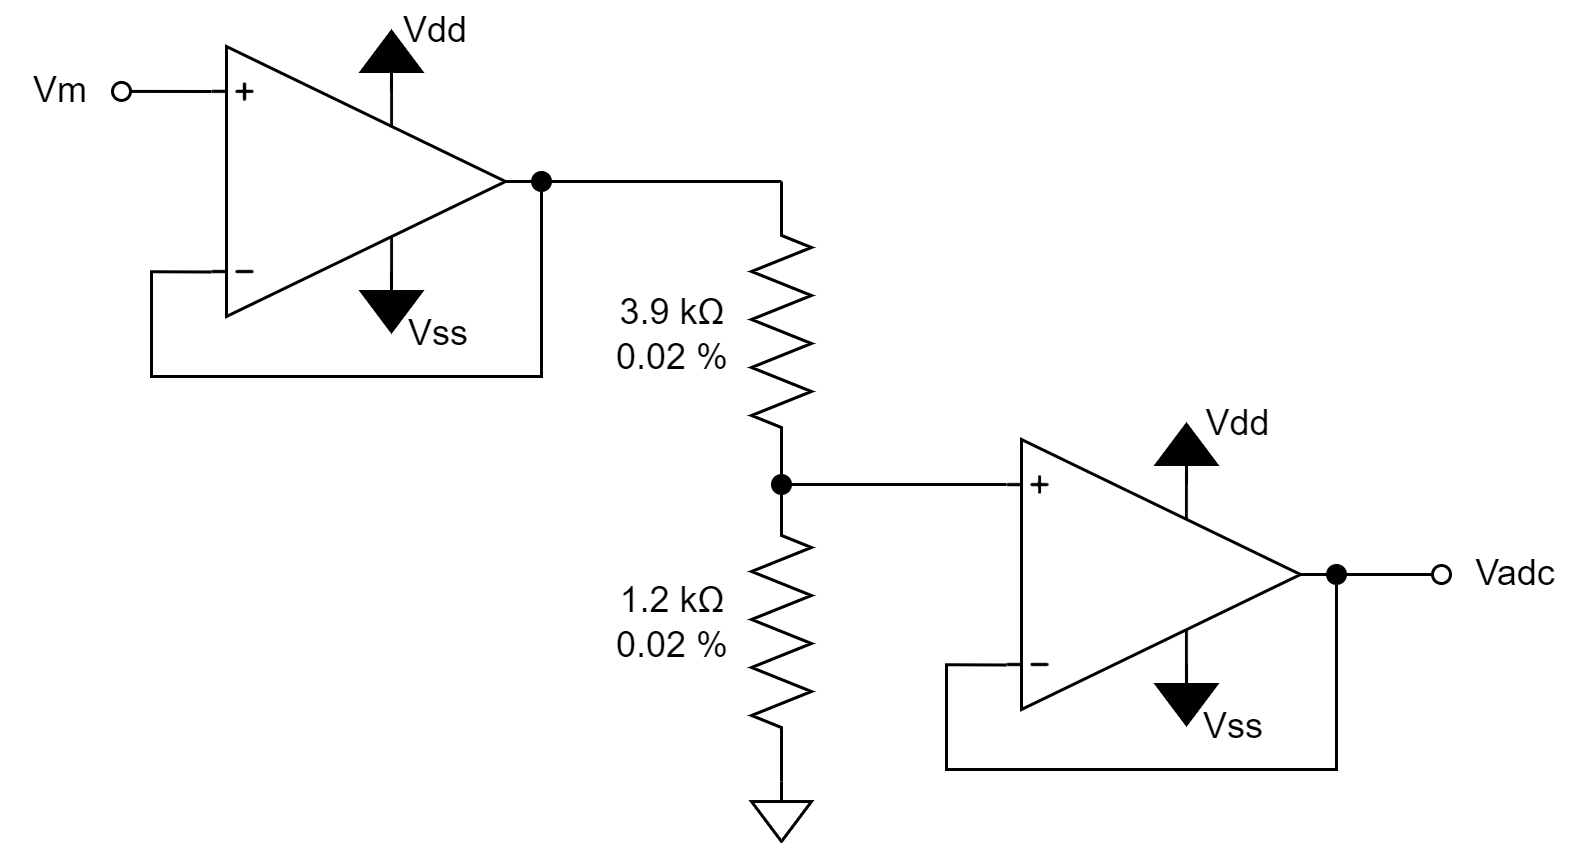
\includegraphics[width=0.5\linewidth]{Figures/opamp_ckt_ert_pcb.png}
\caption{Measurement attenuation circuit}
\label{fig:opamp_ckt}
\end{figure}
To allow larger current signals to be driven through the domain a maximum voltage driving the current source of 20 V is used with an attenuation circuit consisting of two voltage buffers and a voltage divider. The attenuation circuit steps down the voltage with a nominal gain of 0.24 $\pm$ 3\%. The attenuation circuit is duplicated for both differential ADC inputs. This circuit is highly sensitive to any noise, DC offset, or component variation. To combat the sensitivity of this circuit the opamps used [U10, U11] have a low input bias current, and low input DC offset voltage, the resistors used have a low tolerance of $\pm$0.02\%.
\begin{figure}[H]
\centering
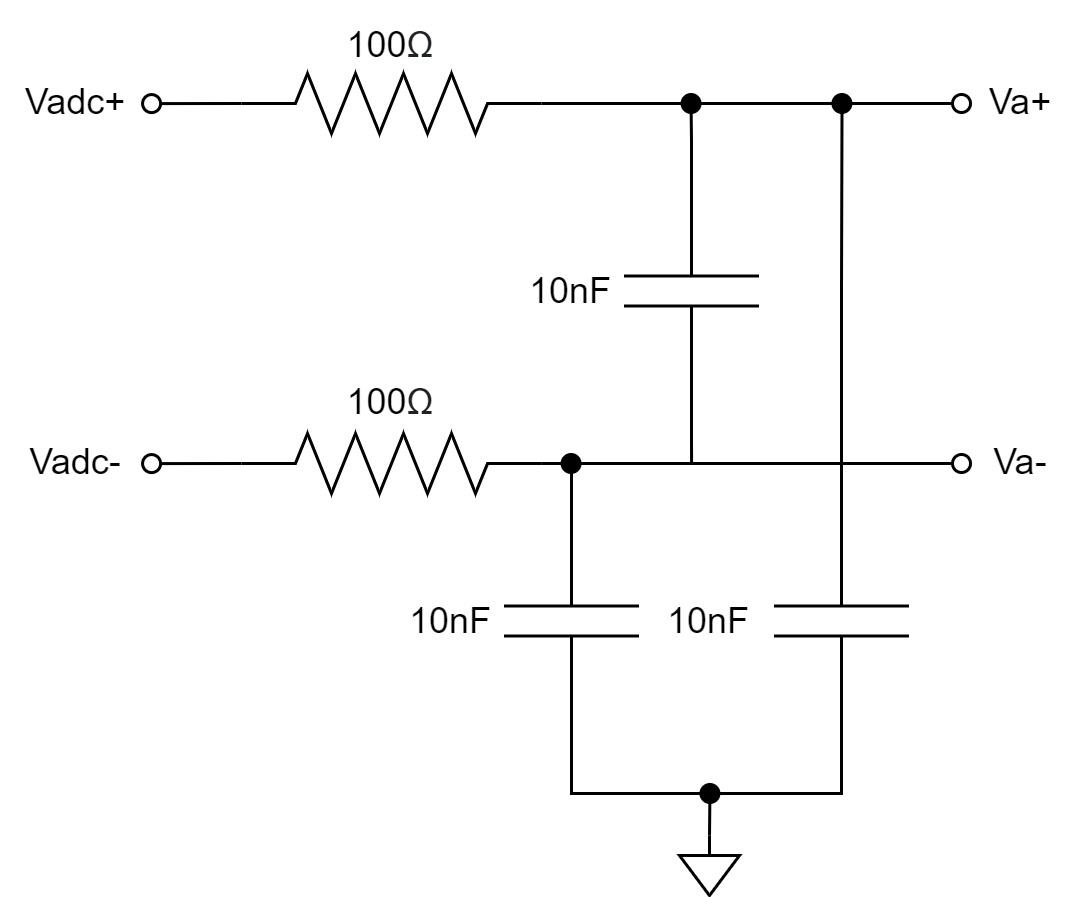
\includegraphics[width=0.4\linewidth]{Figures/adc_filter_ckt.png}
\caption{Passive low-pass filter circuit}
\label{fig:adc_filter_ckt}
\end{figure}
A passive low-pass filter has been placed between the opamp circuit and the ADC input to attenuate ADC input noise. The cutoff frequency for this filter has been set to a value of, 1 MHz allowing for sufficient settling time for the maximum potential ADC sample rate of 512 kSPS.


\subsection{Switching circuit}
% plot the Ron characteristic again VD for a set VDD/VSS??
Previous research has shown the trade-offs with different EIT drive patterns \cite{Tawil2011, Russo2017, Xu2008}. A 4:16 multiplexing circuit allows for a range of EIT switching drive patterns for ERT data acquisition. A multiplexer with a low drain-source on-resistance characteristic for smaller drain voltages has been chosen as the majority of the voltage readings being read through the multiplexer will be nearer to zero than $\pm$Vs.
\begin{figure}[H]
\centering
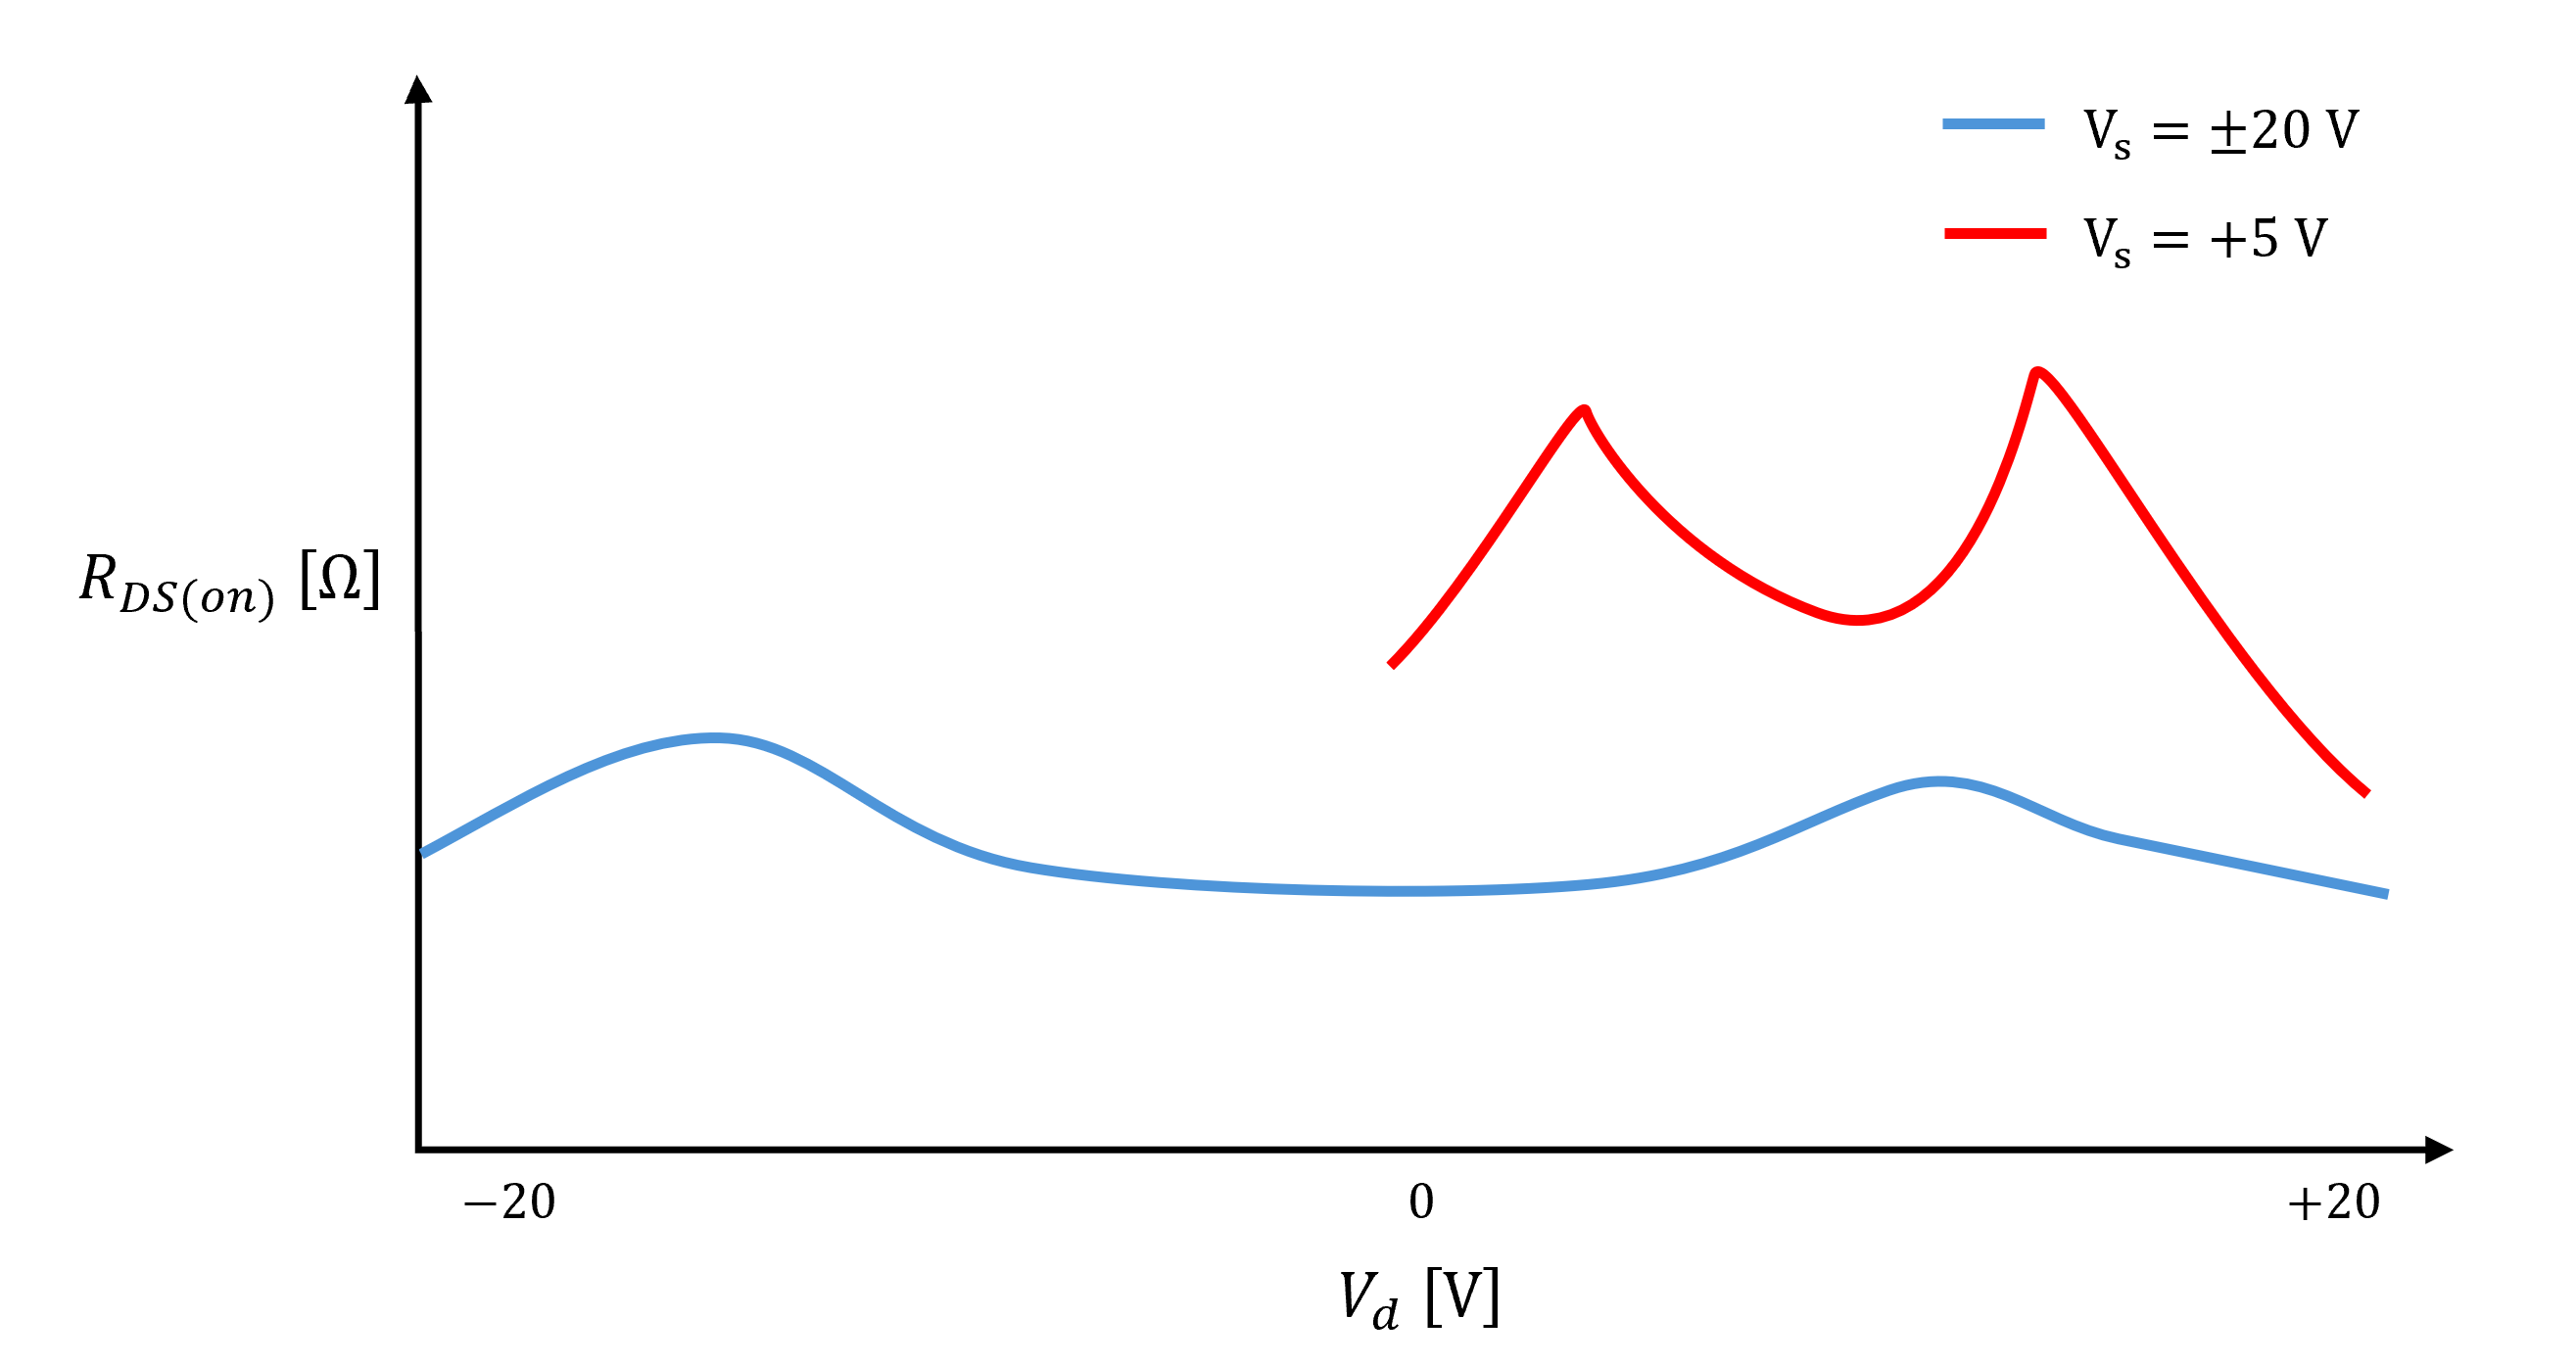
\includegraphics[width=0.7\linewidth]{Figures/mux_r_on_example.png}
\caption{$R_{DS(on)}$ characteristic diagram for a typical multiplexer analogue channel for a dual and single-ended power supply.}\cite{Vishay2024}.
\label{fig:mux_r_on}
\end{figure}

% >> redo this with actual analog switch p-mos n-mos device function. See \href{https://pdfserv.maximintegrated.com/en/an/AN5299.pdf}{AN5299.pdf}

Any variation in the $R_{DS(on)}$ value as a function of $V_D$ or from channel-to-channel will add to the offset noise read by the ADC lowering the resolution of the ERT pressure sensor. This low $R_{DS(on)}$ variation can be seen in Figure \ref{fig:mux_r_on}. The multiplexer used can switch analogue voltage up to $\pm$22 V with a switching time of 200 ns \cite{Vishay2024}.


\subsection{Position control and measurement}
% justify position measurement system. Stepper motors don't skip and can step 0.XX mm increments? Serial-PC connection. Feed it array of strain magnitudes, locations, duration, and strain speed.
To accelerate experiment development a simple and accurate Cartesian force applicator was required. The Prusa MK3s 3D printer was used as the Cartesian force applicator base, because of it's proven reliability as a 3D printer to move in x, y, and z axes with high resolution. The printer head was modified to attach the load applicator module described below. The resolution of the force applicator location under without applying a load is 0.01 mm in each axis. Due to the open-loop nature of control of the stepper motors the resolution at high loads may not be reliable.


\subsection{Force measurement}
The CFA system is designed to be used with soft piezoresistive sensing domains due to loading limitations of the 3D printer frame and the force applicator head design. The force applicator head must be significantly more rigid than the sensing domain being tested to ensure low strain error. 

A static load FEA simulation was completed on the loadcell bracket with the maximum load expected used as 100N. The material of the bracket was PLA with orthotropic material properties. The static simulation used the orthotropic 3D printed PLA properties given by Sosa-Vivas et al. \cite{SosaVivas2023} with Caculix FEM solver \cite{Dhondt2023}. As shown in Figure \ref{fig:FEA_force_aplc} the maximum predicted displacement of an FEM element within the loadcell part was 0.13 mm. If using a sufficiently soft domain and small force applicator this maximum displacement has little effect on the data processed, however this may cause significant error within harder domains and/or larger force applicators. Although the device can operate at 100 N, device operation is recommended below 50 N to decrease the strain error due to force applicator deformation.

\begin{figure}[H]
\centering
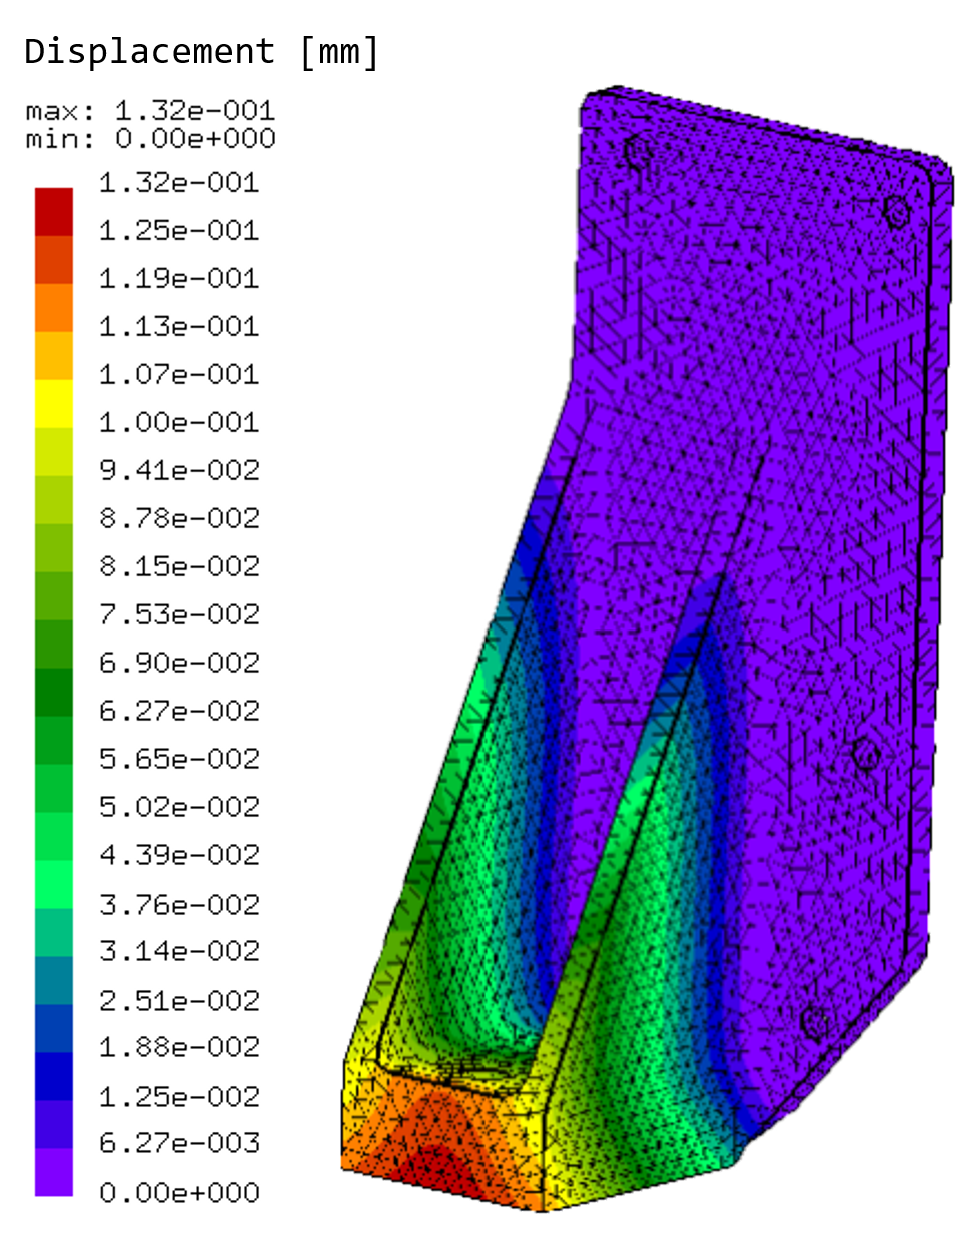
\includegraphics[width=0.45\linewidth]{Figures/fea_ccx_loadcell_bracket.png}
\caption{Static load analysis of the loadcell bracket part [PR9] of maximum allowable load of 100 N showing the magnitude of displacement. }
\label{fig:FEA_force_aplc}
\end{figure}

The TAL220 loadcell used was chosen for the sensing domain material. The CBSR material had an elastic modulus of 100 kPa \cite{Ellingham2024} so that range of strain measurements from 0 - 50\% could be accurately recorded with the given loadcell. The minimum force is on the limit of what can be detected as the loadcell is rated for $\pm$50 mN resolution \cite{HTCSensor2024} across its operating load and temperature range. However the noise of the loadcell was measured to be $\pm$ 2.5 mN during several 15 minute experiments in a 22$\pm$0.7 $\degree$C regulated room. Examples of experiment loading limits are given in Table \ref{tab:cfa_limits}, giving the extreme cases for testing minimum and maximum theoretical strain for 5 and 20 mm diameter force applicator heads on a lower and higher elastic modulus material respectively.
\begin{table}[H]
\hspace{-1cm}
\caption{An example of the extreme parameter limits of two loading experiments showing the minimum and maximum strains limits for 5 mm and 20 mm diameter force applicators and their required forces respectively.}
\label{tab:cfa_limits}

\hspace{-1cm}
\begin{tabular}{|p{0.1\linewidth}|p{0.2\linewidth}|p{0.2\linewidth}|p{0.15\linewidth}|p{0.15\linewidth}|p{0.15\linewidth}|} \hline
	\textbf{Force [N]} &
	\textbf{Force applicator diameter [mm]} &
	\textbf{Force applicator area [$\mathbf{mm^2}$]} &
	\textbf{domain elastic modulus [kPa]} &
	\textbf{Theoretical strain [\%]} &
	\textbf{Theoretical stress [kPa]} \\ \hline
	0.06 &
	5 &
	19.6 &
	60 &
	5.1 &
	3.1 \\ \hline
	50.00 &
	20 &
	314.2 &
	200 &
	79.6 &
	159.2 \\ \hline
\end{tabular}
\end{table}

% TODO: Calcs for the stepper motor strength



\subsection{Sensing domain}
% percolation etc. Mention recommended sonication bath usage.
A core purpose of this system is to test a range of different sensing materials over a range of shapes and sizes. This platform provides a two degree-of-freedom load application over a 220 $\times$ 180 mm area where the load can be applied at heights of 0 to 150 mm.

The example PNEC sensing domain in this work is a carbon black silicone composite. The weight percentage of CB powder in an elastomer matrix to maintain desired mechanical and electrical properties can be tuned as shown in the characterisations completed in literature \cite{D'Asaro2017, Shang2016} and in the previous two chapters. The most desirable piezoresistive characteristics found in these works are near the inflection point of the conductivity versus CB weight percentage plot.

Because of the difference in fabrication processes and degree of dispersion generating variability in the percolation, an iterative trial and error approach using the starting point found in literature was used to get 8 wt \% and 9 wt \% values for CB in SR \cite{D'Asaro2017, Shang2016}. Within this range the material was sufficiently conductive while maintaining mechanical strength through sufficient elastomeric cross-linking. Previous research indicates that there is a weight percentage at which the gauge-factor/piezoresistivity is at a maximum within a similar range used in this work \cite{Dong2017, Yang2020}. The CB particle dispersion can vary throughout a domain depending on various factors in the fabrication process including mixing technique, solvents used, silicone viscosity, particle size, particle agglomerations, amongst other factors \cite{Kalyon2002,Rodgers2010,Lux1993,Xu2016}. Dispersion of carbon black particles was ensured by using a relatively low viscosity silicone of 6,000 mPa.s and a centrifugal planetary mixer a method proven to give more homogeneous dispersion than other traditional mixing techniques \cite{Thinky2010}.



\section{Validation and Characterisation}
\label{sec:Validation and characterisation}
%Demonstrate the operation of the hardware and characterize its performance over relevant critical metrics
%> Demonstrate the use of the hardware for a relevant use case. 
%> If possible, characterize performance of the hardware over operational parameters. 
%> Create a bulleted list that describes the capabilities (and limitations) of the hardware. For example consider descriptions of load, operation time, spin speed, coefficient of variation, accuracy, precision and etc.
To show that the system is functional, the plots produced from an EIT reconstruction of the voltage data and the force measurements can be compared for a correlation. Examples are given below in Figure \ref{fig:rand_recon_result} and \ref{fig:rand_recon_and force_result}, showing localised blobs at the known locations of the force applicator.
\begin{figure}[H]
\centering
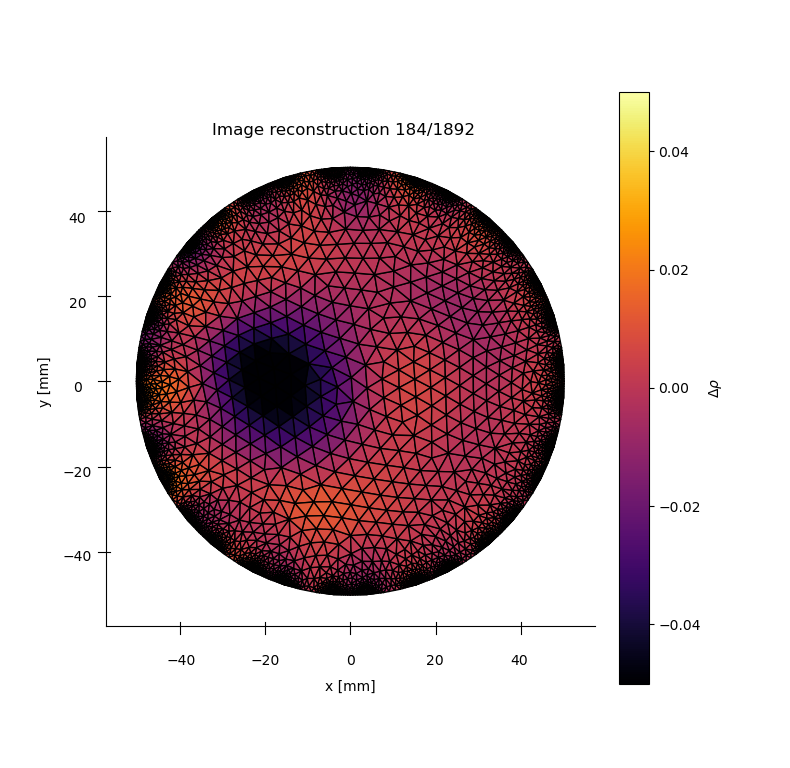
\includegraphics[width=0.49\linewidth]{Figures/DEA1_CBSR_8p_9push_rand10strain_30s_1mA_1_frame184.png}
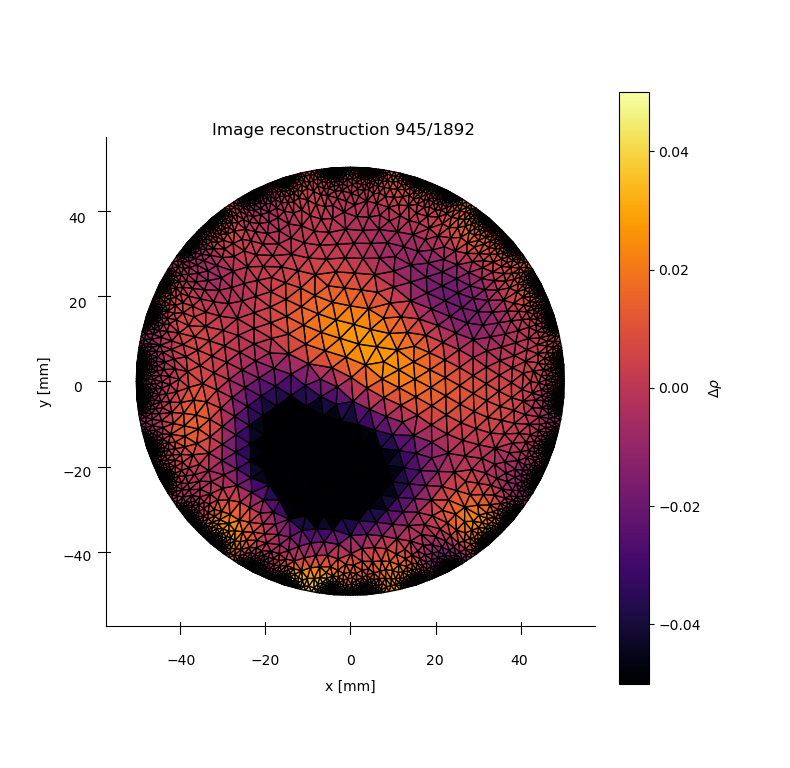
\includegraphics[width=0.49\linewidth]{Figures/DEA1_CBSR_8p_9push_rand10strain_30s_1mA_1_frame945.png}
\caption{Reconstruction frames from a random push test sequence on a 1mm thick 100mm diameter sample. Strain and applied locations (x, y) [mm] - Left: 24\% (-14.8, -3.4). Right: 36\% (-1.9, -21.3)}
\label{fig:rand_recon_result}
\end{figure}
A raw video of this experiment can be seen in the supplementary material \cite{Ellingham2025}. It may be useful to plot the force profile being applied alongside the EIT reconstruction to verify the data is ready for further processing and modelling. 
\begin{figure}[H]
\centering
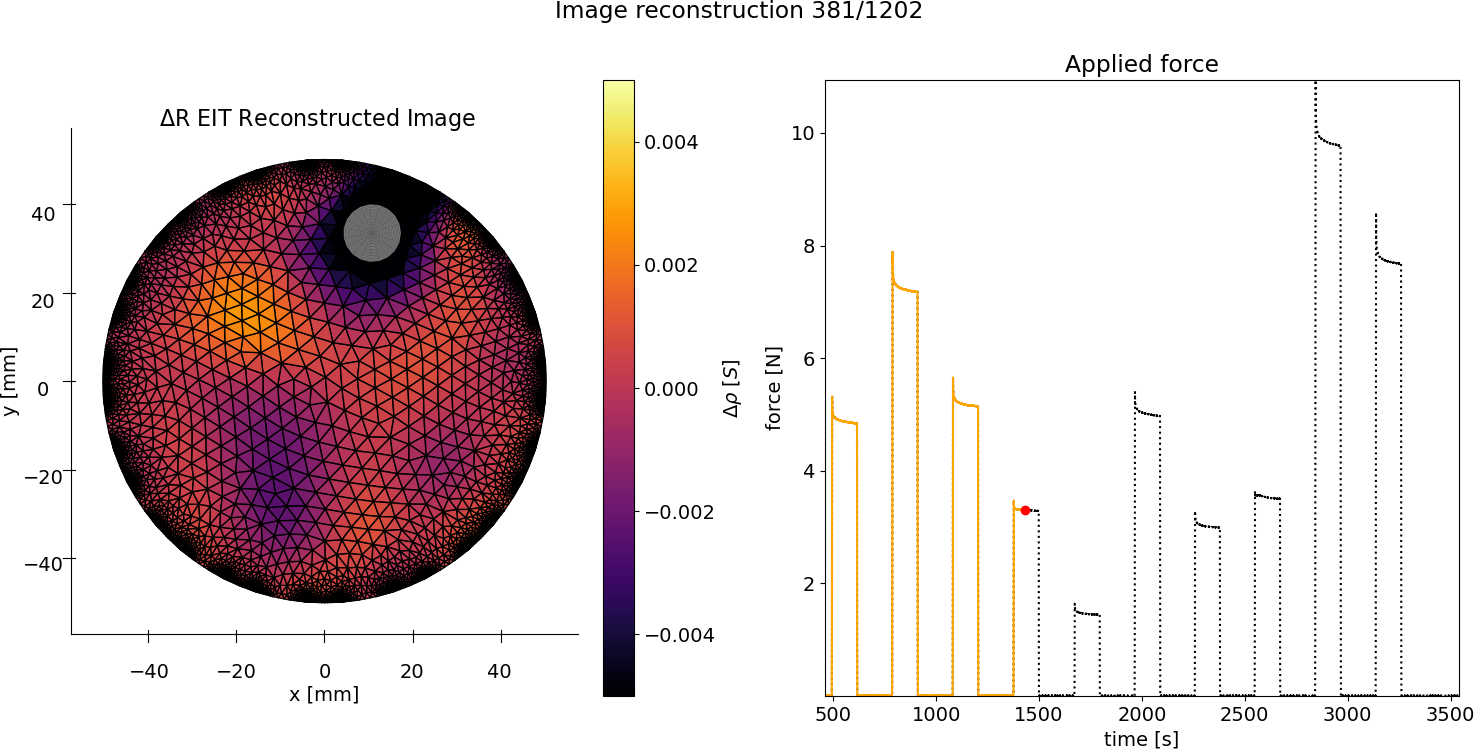
\includegraphics[width=0.9\linewidth]{Figures/CBSR_8p_OG_10push_RAND1_strain_120s_1mA_2_frame381.png}
\caption{Reconstruction frames from a random push test sequence on a CBSR 100mm diameter sample. The white circle representing the force applicator location and the red dot on the force plot showing the captured frame in time.}
\label{fig:rand_recon_and force_result}
\end{figure}

% \subsection{Data collection rate}
% To ensure a range of load event durations can be detected and processed promptly a sufficiently high sample frequency is required.  
% votlage data averaging tradeoff?
% theoretical vs actual sample rate limit. What's the bottle neck? plots?
% USB serial vs Bluetooth vs Wifi

\subsection{Sensor capabilities}

Simultaneous application of multiple loads can be achieved with this system using a multi-head force applicator. It has been shown that multiple touch points can be detected as shown in Figure \ref{fig:multi-touch-eit} the supplementary material and in our previous work \cite{Ellingham2025,Ellingham2022}.
\begin{figure}[H]
\centering
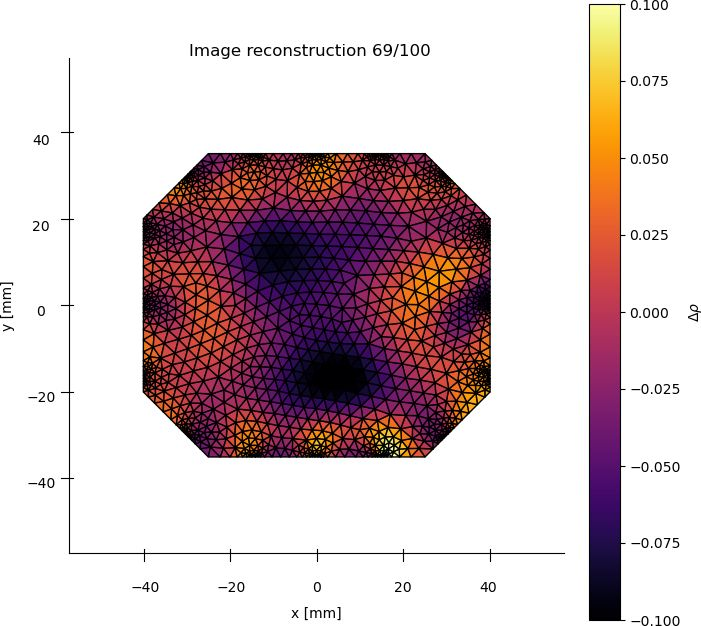
\includegraphics[width=0.45\linewidth]{Figures/multitouch_rect_CBSR_8p_80x70mm_frame69.jpg}% using 1.5mm thick 70 x 80 mm rectangle with 15 mm radius on corners
\hspace{1cm}
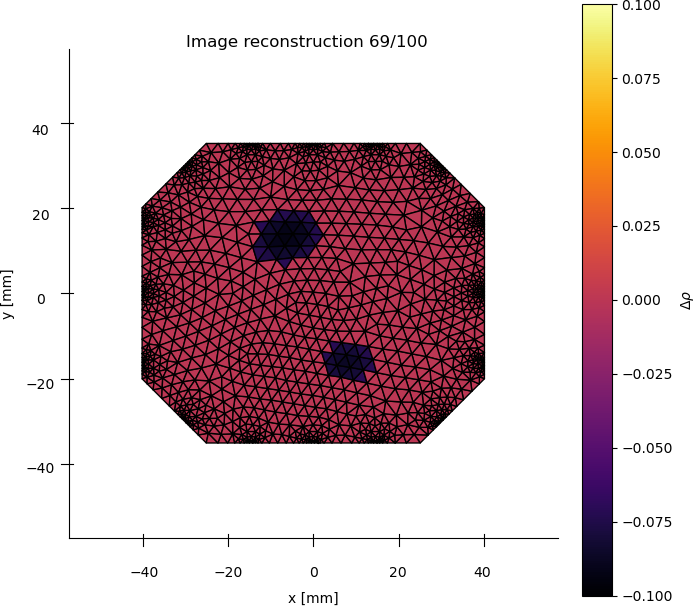
\includegraphics[width=0.45\linewidth]{Figures/multitouch_rect_CBSR_8p_80x70mm_frame69_75p_thresh.png}% using 1.5mm thick 70 x 80 mm rectangle with 15 mm radius on corners
\caption{An EIT reconstruction image of a sensing domain with two loads applied simultaneously. Left: Without threshold filtering. Right: With a 75\% threshold amplitude filter applied.}
\label{fig:multi-touch-eit}
\end{figure}

% >> currently sorting out new mesh for rectangular domain with filleted corners! :D

A major factor constraining the application of EIT-based sensors is the poor frequency response of the material, which limits the detection of rapid successive loads. The system given in this work allows further research into characterising the transient response of a range of sensing domains in 2D. Examples of how transients have been characterised are shown in Figure \ref{fig:2D-transient}
\begin{figure}[H]
\centering
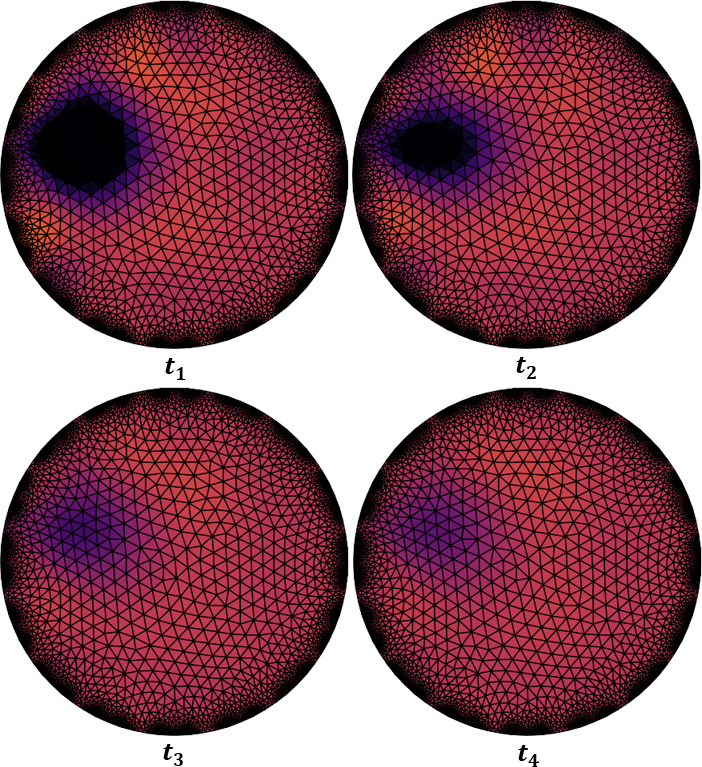
\includegraphics[width=0.35\linewidth]{Figures/res_relax_DEA_EIT_1mm_3load_7kV_1.png}
\hspace{1cm}
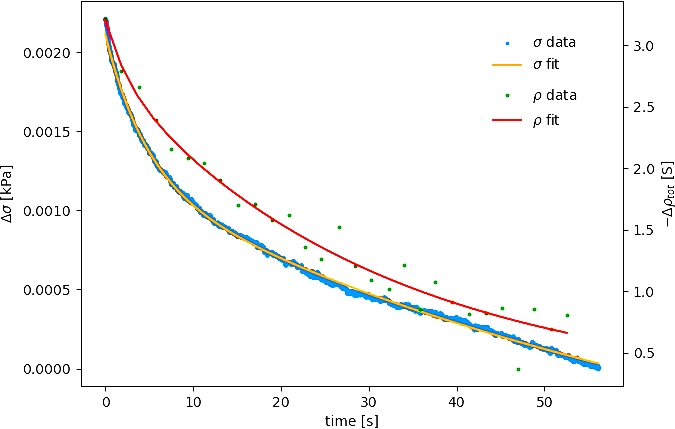
\includegraphics[width=0.54\linewidth]{Figures/2D Push event 0 - CBSR 9 wt 30p strain - 2D compressionv2.jpg}
\caption{Left: Example sequence a resistive relaxation after a loading event at times $t_1$ to $t_4$. Right: Example stress, $\sigma$, and resistive, $\rho$, relaxation plot generated from an ERT CFA experiment given a 30\% strain step input \cite{Ellingham2024}.}
\label{fig:2D-transient}
\end{figure}

The piezoresistivity of a sensing domain can often vary throughout its volume giving unpredictable results if a homogeneous domain is assumed for the pressure mapping sensor. This system can be used to generate map of the piezoresistivity function of a material surface in 2D dimensions.

\section{Discussion}
To move the field of EIT-based soft pressure mapping forward, there is a need to optimise materials for qualities such as pressure sensitivity, homogeneity, electrode connectivity, and dynamic viscoelastic properties.
This CFA automates the testing process with easily changeable spatio-temporal parameters, such as strain magnitude, strain rate, and strain profile. This system standardises the analysis of the pressure mapping by allowing for the EIT reconstructed resistance images to be compared with stress and strain data form the sensing domain material.

The hope for the hardware and software given in this paper is that it will provide a standardised platform for future researchers to use to further quantify the utility of other sensing materials, and compare their performance metrics with standard loading test procedures, as done in our previous work \cite{Ellingham2024}. The ERT sensor and force applicator hardware could be utilised in further research for; 2D piezoresistive material analysis, pressure mapping device characterisation and performance for spatio-temporal performance, dynamic stress sensing performance, piezoresistivity. These research applications are all working towards development for real-world applications such as robotic skin integration, sports sensing, and prosthetics.


% Any non-ideal conditions in the data measurement process affect the EIT reconstruction quality. Several factors affect the data gathered from the system including, temperature, humidity, component variation, electrode noise, power supply noise, ERT circuit component defects, externally generated mechanical vibrations, and ambient electrical noise \cite{?,?,?,?}. 

% >> Could just remove the above paragraph??

% \subsection{Sensitivity Analysis}
% To quantify how robust the system will be over a range of input noise values a range of noise values are added to the system and the resulting noise factors are determined.

\section{Conclusions}
This work has provided the methods and tools to enable further research and development for soft EIT-based pressure sensing systems. The system is low cost, simple to construct, and easy to use. The automation of compression load experiments ensures that experiments are repeatable with quantifiable results and mitigating human error. The automated nature of the CFA device significantly reduces the time to complete a set of experiments and can provide experiment sequences similar to those expected during the real-world application of the sensor. Upon load experiment completion, the system provides clearly formatted raw data files ready for analysis.

A ERT circuit was developed with a data capture frame rate of 12.7 Hz, a drive current of 15 $\mathrm{\mu A}$ - 50 mA at $\pm$22 V, measurement resolution of $\pm$0.3 $\mathrm{\mu V}$. The Cartesian force applicator system developed can apply compressive loads between 0 - 800 mm/min with a xy position resolution of 0.01 mm, and can sense loads from 0 - 100 N with a resolution of $\pm$ 50 mN.
% Current limitations of the system include: lack of closed loop feedback to ensure positional accuracy, the inherently jerky motion of stepper motors, the loadcell resolution for very soft loads, the software interface is could be more user friendly.

Uses of this system vary from 2D piezoresistive material analysis and pressure mapping sensor characterisation. Extensive research has been conducted into one-dimensional (1D) characterisation of piezoresistive materials. However, the characterisation of these materials in two dimensions (2D) has often been overlooked in past literature \cite{Ding2007,Shang2016,Buketov2020,Zhao2013}, often due to the complex and invasive methods required. The device can be used to characterise the electromechanical/piezoresistive properties of a soft thick film material in 2D, quantify EIT reconstruction performance, and generate models predicting localised loads from localised resistance changes.

To push the field of EIT-based pressure mapping forward tools are required to standardise testing and reliably acquire quantifiable data for pressure modelling in different sensing domain materials. A toolbox of hardware and software have been described in this work to make EIT-based pressure mapping realisable for more real-world applications.

Proposed future enhancements of the system include minimising noise and offsets in the signal conditioning ERT circuit, adding an auto-calibration procedure to ensure the ADC and $I_{src}$ circuits operate at the expected resolution, and reducing the PCB size. Also extending the device to drive and read AC signals may mean the complex electrical properties of some PNECs could be used to improve the system performance. The ERT sensor and Cartesian force applicator system described in this work will help transition this technology into real-world applications.


%\afterpage{\blankpage}